% Assignment 4 - Lists, Colors, Figures etc.
% Tarun Konde (2025UCP1811)

\documentclass[11pt,a4paper]{article}

\usepackage[T1]{fontenc}
\usepackage{lmodern}

\usepackage[margin=2.5cm]{geometry}
\usepackage{graphicx}
\usepackage{xcolor}
\usepackage{array}
\usepackage{caption}

\graphicspath{{images/}}

% Custom colour 1: red 200, green 20, blue 200 (0-255 scale).
% In HTML hex this is #C814C8.
\definecolor{mypurple}{RGB}{200,20,200}
% Custom colour 2: 60% red mixed with 40% yellow.
\colorlet{myorange}{red!60!yellow}

\title{Assignment 4 -- Lists, Colors, Figures etc.}
\author{Tarun Konde (2025UCP1811)}
\date{\today}

\begin{document}
\maketitle

\section{Lists}

Following are some technologies that can be used to format content:
\begin{itemize}
    \item \LaTeX
    \item HTML (+CSS)
    \item Markdown
\end{itemize}

You would most likely use \LaTeX{} in the following scenarios:
\begin{enumerate}
    \item To write research papers
    \item To embed math equations within other software (e.g.\ GDocs, HTML etc.)
    \item To create your CV, project reports \& presentations
\end{enumerate}

There are three main categories of electronic markup:
\begin{description}
    \item[Presentational] Used by traditional word-processing systems: binary
        codes embedded within document text that produce the WYSIWYG (``what
        you see is what you get'') effect. e.g.\ Microsoft Word
    \item[Procedural] Markup is embedded in text which provides instructions
        for programs to process the text. e.g.\ \TeX
    \item[Descriptive] Markup is specifically used to label parts of the
        document for what they are, rather than how they should be processed.
        e.g.\ \LaTeX, HTML5
\end{description}

\section{Tables \& Colors}

Code for Table~\ref{tab:lang} is written in this subsection. However, it will
be rendered on a special page because of the \texttt{[p]} placement option.
Changing it to \texttt{[t]}, \texttt{[b]} or \texttt{[h]} moves it to the top,
the bottom, or to this spot. The last row of this table shows the width of
each column.

\begin{table}[p]
    \centering
    \begin{tabular}{|p{2.5cm}|p{2cm}|p{2cm}|p{3.5cm}|}
        \hline
        \textbf{Language} & \textbf{Requires compilation} & \textbf{Output} & \textbf{Use} \\
        \hline
        C/C++       & Yes & Executable & To make apps \\
        \LaTeX      & Yes & PDF        & To make documents \\
        HTML/CSS/JS & No  & Webpage    & To make websites \\
        \hline
        2.5 cm & 2 cm & 2 cm & 3.5 cm \\
        \hline
    \end{tabular}
    \caption{This table should be rendered on a special page.}
    \label{tab:lang}
\end{table}

Colours can be given as numbers in a few models. In RGB each channel is a
number from 0 to 255 (or 0 to 1). HTML writes the same thing in hexadecimal,
so red 200, green 20, blue 200 becomes \texttt{\#C814C8}; CSS also accepts the
numeric form \texttt{rgb(200, 20, 200)}. The first colour below is defined that
way with \verb|\definecolor|, and the second is a 60/40 mix of red and yellow
made with \verb|\colorlet|.

\[
    \textcolor{mypurple}{T(n)} = \textcolor{myorange}{a\,T(n/b)} + \textcolor{mypurple}{f(n)}
\]

\section{Figures}

\subsection{Pictures: rotation \& cropping}

Include the MNIT logo and rotate it appropriately. Also include the MNIT
building picture but crop the sky and make it as wide as the text, as shown in
Figure~\ref{fig:building}.

\begin{figure}[h]
    \centering
    
\includegraphics[width=3.5cm, angle=-15]{mnit_logo.png}
    \caption{MNIT logo}
    \label{fig:logo}
\end{figure}

% trim = left bottom right top. The top value removes the sky.
\begin{figure}
    \centering
    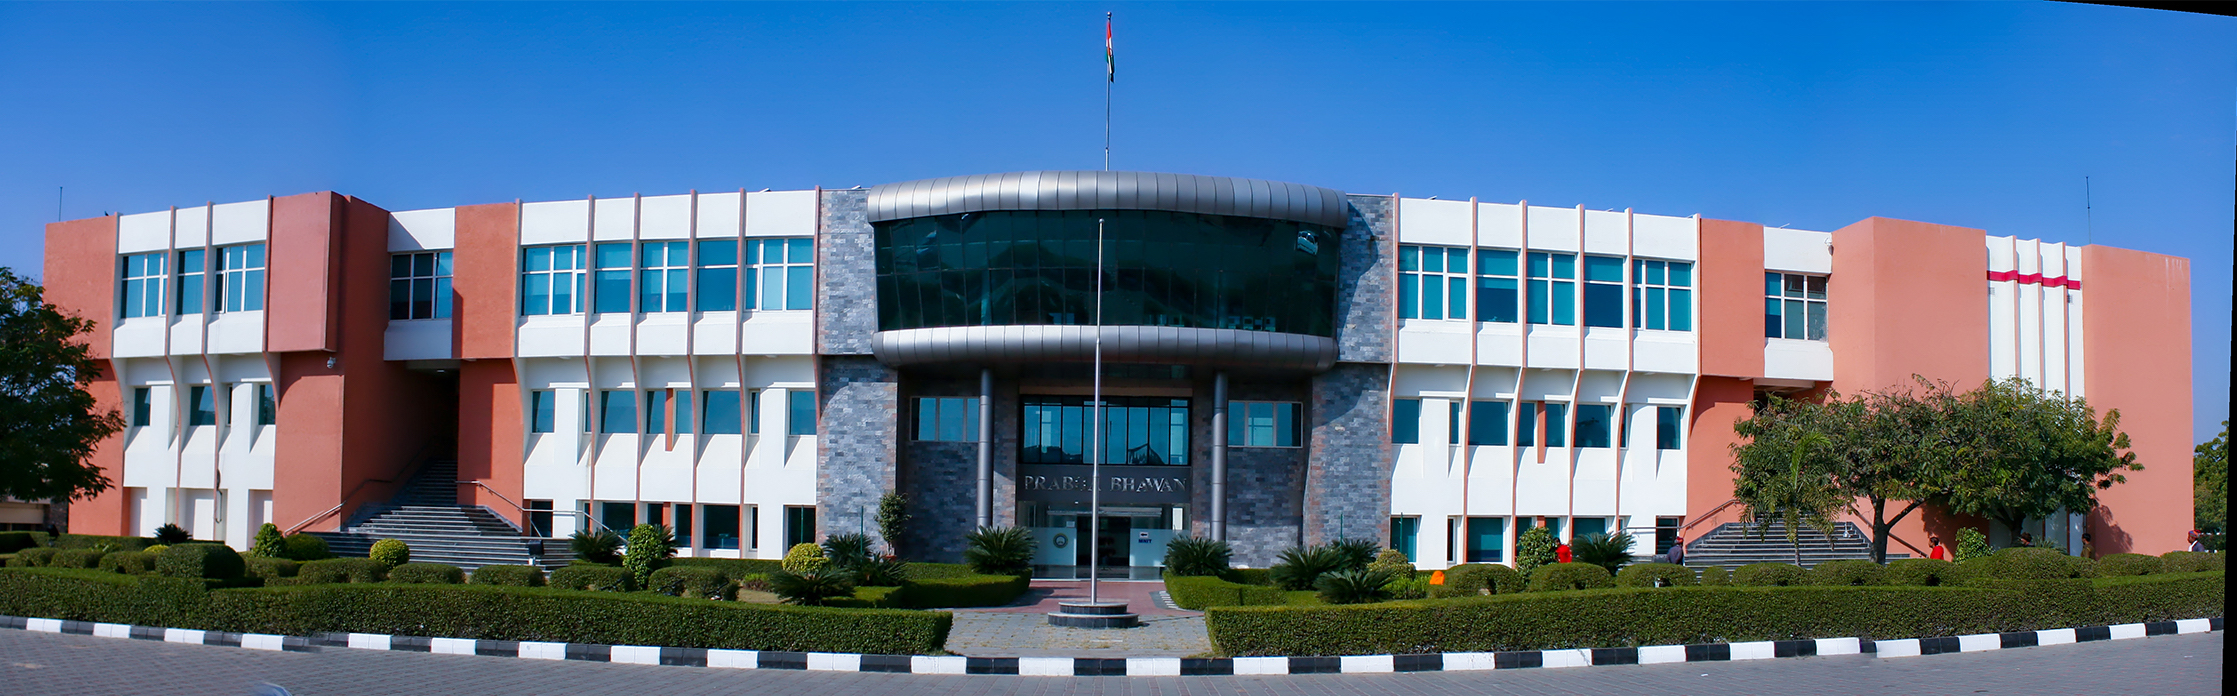
\includegraphics[width=\textwidth, trim={0 0 0 165bp}, clip]{mnit_building.jpg}
    \caption{This is a floating image and can appear anywhere.}
    \label{fig:building}
\end{figure}

\subsection{Multiple images}

This subsection includes two minipages with equal width.

\begin{figure}[h]
    \centering
    \begin{minipage}{0.45\textwidth}
        \centering
        
\includegraphics[width=0.6\linewidth]{mnit_logo.png}
        \caption{This is the first minipage}
        \label{fig:mini1}
    \end{minipage}
    \hfill
    \begin{minipage}{0.45\textwidth}
        \centering
        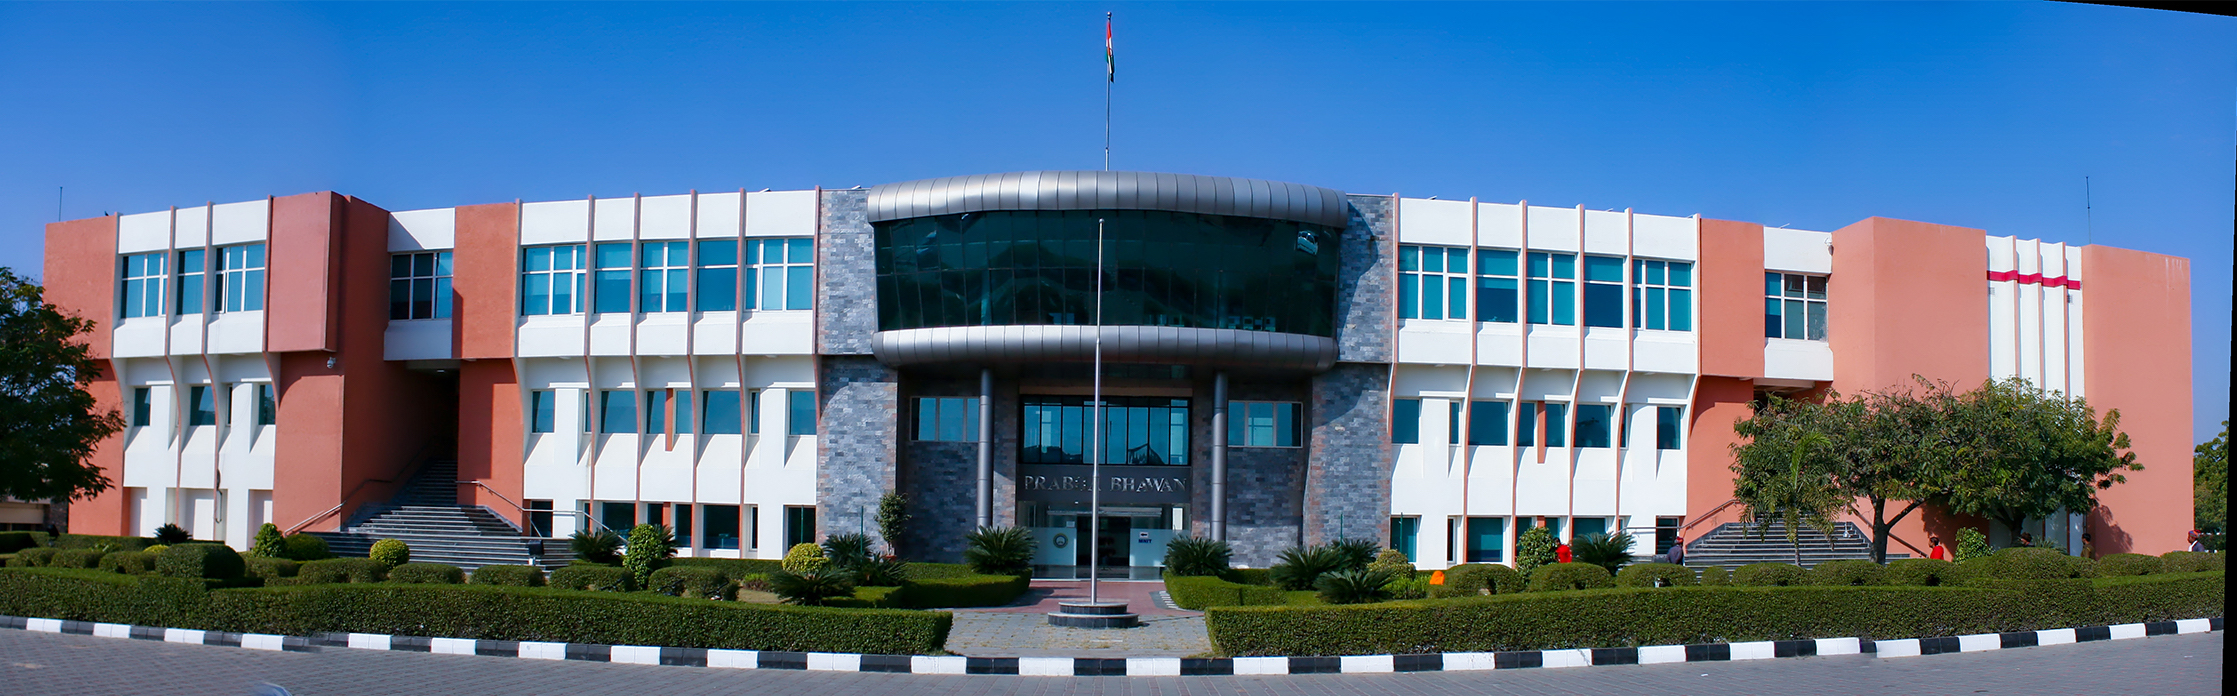
\includegraphics[width=\linewidth]{mnit_building.jpg}
        \caption{This is the second minipage}
        \label{fig:mini2}
    \end{minipage}
\end{figure}

\end{document}
